\documentclass[11pt]{article}

\usepackage[margin=1in]{geometry}
\usepackage{amsmath,amssymb}
\usepackage{booktabs,tabularx,array,multirow}
\usepackage{enumitem}
\usepackage{xcolor}
\usepackage{graphicx}
\usepackage{tikz}
\usetikzlibrary{arrows.meta,positioning,shapes.geometric}
\usepackage[round,authoryear]{natbib}
\usepackage[colorlinks=true,linkcolor=blue!45!black,citecolor=blue!45!black,urlcolor=blue!45!black]{hyperref}
\usepackage{microtype}
\usepackage{caption}
\usepackage{subcaption}
\usepackage{xurl}
\renewcommand{\topfraction}{0.85}
\renewcommand{\textfraction}{0.1}
\renewcommand{\floatpagefraction}{0.8}
\usepackage[section]{placeins}

\newcolumntype{L}{>{\raggedright\arraybackslash}X}
\newcommand{\tbd}{\textcolor{black!45}{--}}

\setlength{\emergencystretch}{1.5em}
\setlist{itemsep=2pt,topsep=4pt}

\title{Can a Year of Production Always Be Completed,\\ and in What Order?\\[4pt] \large A Petri-Net Simulation of the 2018 Philippine Supply and Use Tables}
\author{James Matthew Miraflor\\\small CS 292\\\small First draft: preliminary results}
\date{November 2026}

\begin{document}
\maketitle

\begin{abstract}
A supply and use table records what each industry produced and used during a year, but not the order in which production happened. Following \citet{Bonanno1993,Bonanno1995}, this paper reads the Philippine 2018 Supply and Use Tables as a Petri net, in which an industry can produce only when its inputs are in stock. PSA's tables of 240 products and 240 industries are collapsed to 80 products and 80 industries with PSA's input--output classification. The net is closed into a workflow net whose single case is the year: every industry and every imported product works in 52 equal batches, an opening stock of products is given at the start, and final demand is collected at the end. The paper asks two questions. First, how much opening stock is needed so that every simulated year is completed, and what share of years is completed with less? Second, when the stock is limited, do the years that are completed share a systematic order of industries? Preliminary results from random simulations, with 1{,}000 years for each stock, answer the first question with 26.14 weeks of intermediate use, worth 9.19 trillion pesos: none of 1{,}000 new years stopped with this stock, so fewer than 3 in 1{,}000 years stop, with 95\% confidence. With less stock, fewer years are completed, but not always: 91.9\% of the years are completed with 9 weeks of stock, and only 85.0\% with 13 weeks. At 26.14 weeks industries almost never wait, and the completed years show no order of industries. The next draft looks for an order at a stock where industries wait, records every wait and every stop, and repeats the study with 240 sectors.
\end{abstract}

% =====================================================================
\section{Introduction}\label{sec:intro}
% =====================================================================

The Philippine Statistics Authority (PSA) publishes a supply and use table (SUT) for 2018 \citep{PSA2021SUT}. For 240 products and 240 industries, it records how much each industry produced and how much of each product it used during the year. These are yearly totals. The table does not say in which order production happened, or whether another order would also have worked.

Economics usually reads such a table through equilibrium. In a general equilibrium model, supply and demand meet at a vector of prices, and all the equations of the economy hold at the same time \citep{ArrowDebreu1954}; the input--output model of \citet{Leontief1936} also solves for all outputs at once. In these models nothing happens before or after anything else: the equations are solved as if instantly. This paper takes a different view. It treats production as many \emph{concurrent} processes, that is, processes whose order is not fixed in advance: each one can run whenever its inputs are in stock, and its outputs become inputs for others. Both views are timeless when compared with dynamic models of the economy, in which production takes time and stocks pass from one period to the next \citep{KydlandPrescott1982}: neither view has a calendar. But they show different things. The equilibrium view asks whether the flows of the year are consistent with one another. The concurrent view asks whether the year can be completed step by step from a given stock, and in which order.

\citet{Bonanno1993,Bonanno1995} showed how to study this. A production system described by an input matrix and an output matrix can be read as a Petri net: products are places, processes are transitions, and the products in stock are tokens. A process can run only if all its inputs are in stock. In such a net the order of production matters: from the same stock, one order can continue while another stops.

This paper builds such a net from the 2018 SUT, collapsed to 80 products and 80 industries, and closes it into a \emph{workflow net} \citep{vanderAalst1997,vanderAalst1998}: a net with one start and one end, whose single case is the year. It asks two questions.
\begin{enumerate}[label=\textbf{Q\arabic*.},leftmargin=*]
\item \textbf{Stock.} How much opening stock is needed so that every simulated year is completed? For smaller stocks, what share of simulated years is completed?
\item \textbf{Order.} When the stock is limited, do the years that are completed share a systematic order of industries?
\end{enumerate}

The table does not report stock levels, so the opening stock is the experimental variable, measured in weeks of intermediate use. The year is too large to check exactly, so the paper uses random simulation. Completing every simulated year is the practical test of the property that matters: that the year can be completed in every order of its batches that the stock allows. A single stopped year proves that some order fails. When all 1{,}000 simulated years at a stock chosen in advance are completed, the chance that a random run stops at that stock is below 3 in 1{,}000, with 95\% confidence. With 52 weeks of stock, every order completes, because the stock of every product then covers its use in the whole year.

The model describes the table, not the calendar. Batches are equal parts of each industry's year, with no seasons, and the simulation lets batches run in any order that the stock allows. The results therefore describe what the input structure of the 2018 table requires. They do not describe how the Philippine economy actually scheduled its production.

\paragraph{Related work.} Bonanno's examples are small and built by hand, and his nets have no end; we are not aware of an application of his model to a national SUT. \citet{MolinaGutierrez2015} write the Leontief model as a Petri net to simulate the timing of production cycles, using a symmetric input--output table. Other methods derive an order of industries from the structure of an input--output table: structural path analysis \citep{DefournyThorbecke1984}, upstreamness \citep{Antras2012} and triangularization \citep{Fukui1986}. This paper looks instead for an order in time that limited stock creates. A comparison of the two kinds of order is left for later work.

\paragraph{Preliminary findings.} With the 80-sector table and 52 batches (Section~\ref{sec:results}):
\begin{itemize}[leftmargin=*]
\item \textbf{Q1.} None of 1{,}000 new simulated years stopped with 26.14 weeks of stock (9.19 trillion pesos, about half of a year's intermediate use), so fewer than 3 in 1{,}000 years stop at this stock, with 95\% confidence.
\item \textbf{More stock is not always better.} 91.9\% of the years are completed with 9 weeks of stock, but only 85.0\% with 13 weeks; no year stopped with 17 or 22 weeks, but 5 of 1{,}000 stopped with 26 weeks.
\item \textbf{Q2.} At 26.14 weeks, industries almost never wait, and the completed years show no order of industries.
\end{itemize}

Section~\ref{sec:example} shows both questions in a small example. Section~\ref{sec:terms} defines the Petri-net terms, Section~\ref{sec:data} describes the data and how they are collapsed to 80 sectors, and Section~\ref{sec:net} builds the net. Sections~\ref{sec:sim} and~\ref{sec:analysis} describe the simulations and the analysis of the firing logs, and Section~\ref{sec:code} describes the code. Section~\ref{sec:results} gives the preliminary results and Section~\ref{sec:discussion} discusses them. Section~\ref{sec:next} lists the next steps, among them the study with 240 sectors, and Section~\ref{sec:conclusion} concludes.

% =====================================================================
\section{A small example}\label{sec:example}
% =====================================================================

The example has three products (crops, goods and power) and three industries (Farming, Factory and Power plant). Each industry runs 3 batches in the year. Table~\ref{tab:recipes} shows what one batch uses and makes. A batch can run only if the stock holds all of its inputs; it then takes its inputs from the stock and adds its output.

\begin{table}[htbp]
\centering\small
\caption{The small example: what one batch of each industry uses and makes.}
\label{tab:recipes}
\begin{tabular}{@{}lcccc@{}}
\toprule
Batch & Crops used & Goods used & Power used & Output\\
\midrule
Farming & 1 & 1 & 2 & 6 crops\\
Factory & 2 & 1 & 2 & 6 goods\\
Power plant & 1 & 2 & 1 & 6 power\\
\midrule
One batch of each & 4 & 4 & 5 & 6 of each\\
\bottomrule
\end{tabular}
\end{table}

\paragraph{Same stock, two orders.} Start with the stock (crops, goods, power) $=(4,4,5)$, exactly the inputs of one batch of each industry.
\begin{itemize}[leftmargin=*]
\item \emph{Order A}: Power plant, Farming, Factory, repeated three times. After each round the stock is $(6,6,6)$, then $(8,8,7)$, then $(10,10,8)$. All 9 batches run. The final stock is the opening stock plus $(6,6,3)$, which is what the year delivers to final users.
\item \emph{Order B}: Factory, Factory. The stock becomes $(2,9,3)$ and then $(0,14,1)$. No crops are left, and every batch needs crops, so nothing can run. Seven batches are left, and the year stops.
\end{itemize}
Both orders start from the same stock and have the same recipes. One completes the year; the other stops.

\paragraph{The stock decides how many orders complete.} The 9 batches can be arranged in $9!/(3!\,3!\,3!)=1{,}680$ orders. Table~\ref{tab:toystock} shows, for several opening stocks, how many of these orders complete, and the share of random runs that complete when each step picks one of the possible batches at random. Each stock is also given in batches of use: $(4,4,5)$ is exactly the input of one batch of each industry, and $(10,10,13)$ is 2.5 such batches, rounded up. Section~\ref{sec:stock} measures the stock of the 2018 net in the same way.

\begin{table}[htbp]
\centering\small
\caption{The small example: completion by opening stock (exact counts).}
\label{tab:toystock}
\begin{tabular}{@{}ccccc@{}}
\toprule
Opening stock & In batches & Orders that complete & Share of random runs & Every order\\
(crops, goods, power) & of use & (of 1{,}680) & that complete & completes?\\
\midrule
$(3,3,4)$ & 0.75 & 0 & 0.00 & No\\
$(4,4,5)$ & 1 & 360 & 0.21 & No\\
$(6,6,8)$ & 1.5 & 1{,}122 & 0.57 & No\\
$(9,9,12)$ & 2.25 & 1{,}620 & 0.84 & No\\
$(10,10,13)$ & 2.5 & 1{,}680 & 1.00 & Yes\\
\bottomrule
\end{tabular}
\end{table}

With $(10,10,13)$, every order completes. More stock does not always help, however: from $(10,10,9)$ no run stops, but from $(10,10,10)$ some runs stop. With 10 units of power, the order Farming, Farming, Farming, Factory, Factory uses all the power, and then neither the last Factory batch nor the Power plant can run. With 9 units, the second Factory batch cannot run, so the Power plant runs instead and the year continues. Even along the scale of Table~\ref{tab:toystock}, where the stock is a multiple of one batch of use, rounded up, the share can fall: 63\% of random runs complete from $(6,6,7)$, but 57\% from $(6,6,8)$. Each stock level must therefore be studied on its own.

\paragraph{An order among the completed years.} At $(6,6,8)$, 35\% of the completed runs reached a step at which some industry had to wait for an input. In the completed runs, the Power plant's $n$-th batch comes before the Factory's $n$-th batch in 57\%, 53\% and 53\% of cases ($n=1,2,3$), and Farming batches also tend to come before Factory batches. The Factory, which needs the most inputs, tends to run last. At $(10,10,13)$ no batch ever waits and every run completes, and every such share is exactly 50\%: there is no order. Waiting is not the only source of an order, however. At $(10,10,10)$ no completed run waits, but 10.5\% of the runs stop, and in the completed runs the Power plant's first batch comes before the Factory's first batch in 56\% of cases: the runs in which the Factory ran early are the ones that stopped, so they are missing from the completed runs. An order among the completed years can therefore come from waiting, or from the selection of the years that complete.

In the small example, on the scale of Table~\ref{tab:toystock}, the smallest stock at which every year is completed is $(10,10,13)$, or 2.5 batches of use, while with $(9,9,12)$, 84\% are. Off this scale, a smaller stock can also complete every year: $(10,10,9)$ does. The answer to Q2 depends on the stock: at $(10,10,13)$ there is no order, while at $(6,6,8)$ the Factory tends to run last. The paper asks the same two questions of the 2018 table.

% =====================================================================
\section{Petri nets and workflow nets}\label{sec:terms}
% =====================================================================

Table~\ref{tab:terms} lists the terms used in this paper \citep{Murata1989,vanderAalst1997}.

\begin{table}[htbp]
\centering\small
\caption{Petri-net terms and their meaning in this paper.}
\label{tab:terms}
\begin{tabularx}{\textwidth}{@{}lL@{}}
\toprule
Term & Meaning\\
\midrule
Place & A product (drawn as a circle). The net also has a few bookkeeping places, such as counters.\\
Transition & A batch of an industry, an import delivery, or the opening or closing of the year (drawn as a rectangle).\\
Token & One unit of a product in stock.\\
Marking & The stock of every place at a given moment.\\
Enabled & A transition is enabled when all its inputs are in stock.\\
Firing & Running an enabled transition once: its inputs are taken away and its outputs are added.\\
Run & A sequence of firings, each made from the marking left by the one before.\\
Deadlock & A marking at which no transition is enabled. A deadlock with batches still left is \emph{premature}: the year stops.\\
Workflow net & A net with one start place and one end place, in which every place and transition lies on a path from start to end. One token in the start place is one case (here, the year).\\
Sound & From every marking that a run can reach, the end can still be reached; when the end is reached, nothing is left elsewhere; and every transition can fire in some run.\\
\bottomrule
\end{tabularx}
\end{table}

If every transition of the net fires a fixed number of times, as in this paper, the state equation $z'=z_0+(B-A)x$ gives the final marking $z'$ from the opening marking $z_0$ and the firing counts $x$, whatever the order \citep{Bonanno1995}. The state equation checks the totals, not the order, so it cannot tell whether an order exists that completes the plan.

Soundness can be decided, but for a net of this size the set of reachable markings is far too large to explore \citep{vanderAalst2011}. The paper therefore uses random runs: at each step, one enabled transition is chosen at random, and every enabled transition has a positive chance. Two facts follow.
\begin{itemize}[leftmargin=*]
\item A single run that stops early \emph{proves} that the net is not sound.
\item If all $R$ runs at a stock chosen in advance complete, the chance that a random run stops is below $3/R$ with 95\% confidence \citep{HanleyLippmanHand1983}. This is evidence for soundness, not a proof.
\end{itemize}

% =====================================================================
\section{Data}\label{sec:data}
% =====================================================================

The data are PSA's 2018 Supply and Use Tables \citep{PSA2021SUT,PSA2021Release}, in million pesos at current prices. The supply table $V$ gives $v_{ij}$, the output of product $i$ by industry $j$, and the imports $M_i$ of each product. The use table $U$ gives $u_{ij}$, the use of product $i$ by industry $j$, the final demand $f_i$ for each product, and the value added of each industry.

\paragraph{From 240 to 80 sectors.} PSA publishes the two tables with 240 products and 240 industries. Product $j$ and industry $j$ have the same code: for example, product 001 is palay, and industry 001 is the growing of palay. PSA's 2018 Input-Output Industry Classification \citep{PSA2021Class} puts each of the 240 codes into one of 80 groups. The tables are collapsed by adding up the rows (products) and the columns (industries) that belong to the same group; products and industries are grouped in the same way, and imports are added up by product group. For example, the 23 food-manufacturing industries (codes 046 to 068) become one industry, Manufacture of food products, and their 23 products become one product. In 47 of the 80 groups there is a single code, such as palay or electricity; the largest groups are food products (23 codes) and professional, scientific, technical, administrative and support services (17 codes). With $G_{ig}=1$ if code $i$ belongs to group $g$ and $G_{ig}=0$ otherwise,
\begin{equation}
V^{80}=G^{\top}VG,\qquad U^{80}=G^{\top}UG,\qquad M^{80}=G^{\top}M .
\end{equation}
Collapsing only adds values, so every total and every accounting identity stays the same. The collapsed tables were built in a workbook and checked against a second collapse made directly from PSA's 240-sector tables: the two agree to the last digit of floating-point arithmetic (largest relative difference below $10^{-15}$). From here on, the paper uses the 80-sector tables, and $V$, $U$ and $M$ denote them.

\begin{itemize}[leftmargin=*]
\item \textbf{The table balances.} For every product, output plus imports equals intermediate use plus final demand. For the economy, value added (18.27 trillion pesos) plus imports (7.66) equals final demand (25.93). These are the two ends of the year.
\item \textbf{Several products per industry.} 79 of the 80 industries supply more than one product. Each industry is treated as one process that makes its observed mix of products in fixed proportions.
\item \textbf{Imports.} 67 of the 80 products are imported and 13 are not. The use table does not separate domestic and imported units of a product.
\item \textbf{Values, not physical units.} A token is a unit of product value, measured in pesos.
\end{itemize}

% =====================================================================
\section{The year-plan workflow net}\label{sec:net}
% =====================================================================

\subsection{Batches}

The year of each industry is divided into $N=52$ equal \emph{batches}. One batch of industry $j$ uses $1/N$ of the industry's yearly inputs, $U_{\cdot j}/N$, and makes $1/N$ of its yearly outputs, $V_{\cdot j}/N$. Each imported product arrives in $N$ equal deliveries of $M_i/N$. The \emph{plan} of the year is that every batch and every delivery fires exactly once: $N(80+67)=7{,}644$ firings.

We use 52 batches because 52 maps easily to weeks: a batch is one fifty-second of an industry's year, the size of one week of its output. But a batch is only a size, not a date. The net has no calendar: any batch may run at any moment at which its inputs are in stock.

\subsection{Places and transitions}

Figure~\ref{fig:wfnet} shows the net. It has a start place, an end place, one place for each of the 80 products, and bookkeeping places that limit each industry and each imported product to $N$ firings. It has four kinds of transition.
\begin{itemize}[leftmargin=*]
\item The \textbf{opening} takes the token from the start place and delivers the opening stock $z_0$ of products, the year's labor and capital services of each industry ($N$ tokens, one per batch), and the year's import deliveries ($N$ tokens per imported product).
\item An \textbf{industry batch} takes one labor-and-capital token and its inputs, and delivers its outputs.
\item An \textbf{import delivery} takes one import token and delivers one delivery of the product.
\item The \textbf{closing} fires only after every batch and delivery has fired. It takes the year's final demand together with the opening stock, $z_0+N\tilde f$, and puts one token into the end place.
\end{itemize}
Labor, capital and imports therefore enter at the start, and final demand leaves at the end. The national accounts make these two ends balance.

\begin{figure}[htbp]
\centering
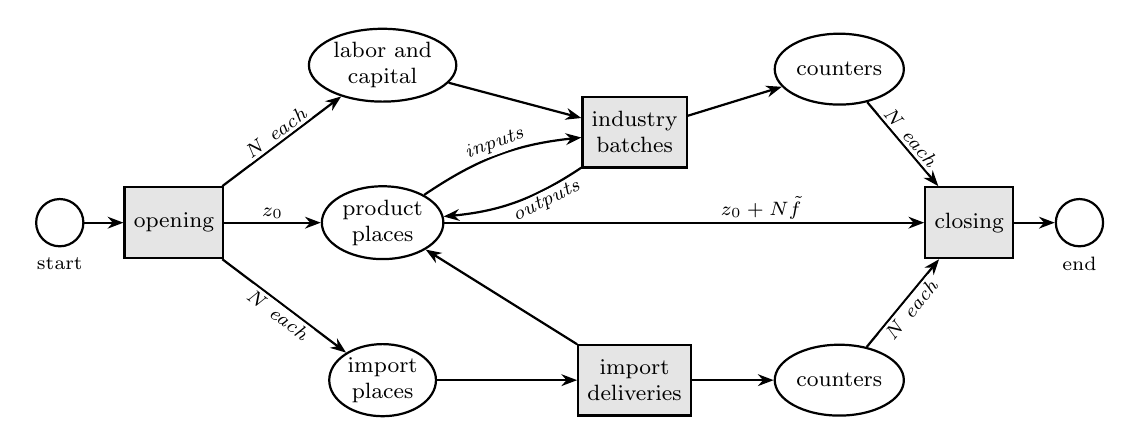
\begin{tikzpicture}[
  pl/.style={ellipse,draw,thick,align=center,font=\footnotesize,inner sep=1pt,minimum height=9mm},
  tr/.style={rectangle,draw,thick,fill=black!10,align=center,font=\footnotesize,minimum height=9mm},
  arr/.style={-{Stealth[length=2mm]},thick},
  lab/.style={font=\scriptsize\itshape,fill=white,inner sep=1pt}
]
\node[circle,draw,thick,minimum size=6mm,label=below:{\scriptsize start}] (i) at (0,0) {};
\node[tr] (st) at (1.45,0) {opening};
\node[pl] (F) at (4.1,2.0) {labor and\\capital};
\node[pl] (P) at (4.1,0) {product\\places};
\node[pl] (I) at (4.1,-2.0) {import\\places};
\node[tr] (Ind) at (7.3,1.15) {industry\\batches};
\node[tr] (Imp) at (7.3,-2.0) {import\\deliveries};
\node[pl] (Di) at (9.9,1.95) {counters};
\node[pl] (Dm) at (9.9,-2.0) {counters};
\node[tr] (en) at (11.55,0) {closing};
\node[circle,draw,thick,minimum size=6mm,label=below:{\scriptsize end}] (o) at (12.95,0) {};
\draw[arr] (i) -- (st);
\draw[arr] (st) -- node[lab,above,sloped] {$N$ each} (F);
\draw[arr] (st) -- node[lab,above] {$z_0$} (P);
\draw[arr] (st) -- node[lab,below,sloped] {$N$ each} (I);
\draw[arr] (F) -- (Ind);
\draw[arr] (P) to[bend left=14] node[lab,above,sloped] {inputs} (Ind);
\draw[arr] (Ind) to[bend left=14] node[lab,below,sloped,pos=0.3] {outputs} (P);
\draw[arr] (I) -- (Imp);
\draw[arr] (Imp) -- (P);
\draw[arr] (Ind) -- (Di);
\draw[arr] (Imp) -- (Dm);
\draw[arr] (P) -- node[lab,above,pos=0.66] {$z_0+N\tilde f$} (en);
\draw[arr] (Di) -- node[lab,above,sloped] {$N$ each} (en);
\draw[arr] (Dm) -- node[lab,below,sloped] {$N$ each} (en);
\draw[arr] (en) -- (o);
\end{tikzpicture}
\caption{The year-plan workflow net. Small circles are the start and end places, ellipses are groups of places, and grey rectangles are groups of transitions. The closing can fire only when every counter holds $N$ tokens, that is, when every batch and delivery has fired.}
\label{fig:wfnet}
\end{figure}

\subsection{Whole-number units}

Tokens are whole numbers, but the flows range from thousands of pesos to billions. Each product $i$ therefore gets its own unit $s_i$, a power of ten chosen so that a typical flow of the product per batch is about $10^5$ units:
\begin{equation}
s_i=10^{\operatorname{round}(\log_{10}\chi_i)-5},
\end{equation}
where $\chi_i$ is the median of the product's positive flows per batch (its use, supply and import cells). The batch weights are the flows in these units, rounded to whole numbers with halves rounded up:
\begin{equation}
\tilde a_{ij}=\operatorname{round}\!\left(\frac{u_{ij}}{N s_i}\right),\qquad
\tilde b_{ij}=\operatorname{round}\!\left(\frac{v_{ij}}{N s_i}\right),\qquad
\tilde m_i=\operatorname{round}\!\left(\frac{M_i}{N s_i}\right).
\end{equation}
Final demand per batch is what the rounded table leaves over,
\begin{equation}
\tilde f_i=\textstyle\sum_j\tilde b_{ij}+\tilde m_i-\sum_j\tilde a_{ij},
\label{eq:balance}
\end{equation}
so that a completed year balances exactly: over the plan, product $i$ gains $N(\sum_j\tilde b_{ij}+\tilde m_i)$ and loses $N\sum_j\tilde a_{ij}$, so the closing finds $z_0+N\tilde f$, whatever the order. Table~\ref{tab:rounding} shows that rounding changes almost nothing.

\begin{table}[htbp]
\centering\small
\caption{Effect of rounding to whole units ($N=52$, 80 sectors).}
\label{tab:rounding}
\begin{tabular}{@{}lc@{}}
\toprule
Input links (positive $u_{ij}$) & 2{,}696\\
Input links that round to zero & 22 (0.82\%)\\
Share of the value of inputs on those links & $3.6\times10^{-8}\,\%$\\
Output links, import deliveries or whole input sets lost & 0\\
Products with negative $\tilde f_i$ & 0\\
Largest whole number in the net & $5.7\times10^{9}$\\
\bottomrule
\end{tabular}
\end{table}

\subsection{Opening stock}\label{sec:stock}

A \emph{week of use} of a product is a quantity: one fifty-second of the year's use of that product by all industries, which is the input of one batch of every industry. The opening stock gives every product the same number of weeks, $w$:
\begin{equation}
z_{0i}(w)=\Big\lceil w\textstyle\sum_j\tilde a_{ij}\Big\rceil .
\label{eq:stock}
\end{equation}
One week of stock is worth 0.35 trillion pesos, and 52 weeks, the whole year's use, are worth 18.27 trillion pesos. The opening stock is working capital: the closing returns it. With $w=52$, the stock of each product at the start is at least its use in the whole year, so no batch ever has to wait for an input, and every order completes.

% =====================================================================
\section{Simulation design}\label{sec:sim}
% =====================================================================

\paragraph{Random runs.} A run starts after the opening has fired. At each step, the possible steps are the industries with batches left whose inputs are all in stock, and the imported products with deliveries left. One of them is chosen with equal chances and fired. The run continues until nothing is possible; it has then either completed the plan or stopped. The equal chances are a way to sample orders; they do not describe how firms decide.

\paragraph{Completion at each stock (Q1).} For each $w\in\{2,4,9,13,17,22,26,35,52\}$ weeks (0.5, 1, 2, 3, 4, 5, 6, 8 and 12 months, rounded to whole weeks), 1{,}000 runs are made. The paper reports the share of runs that complete, with a 95\% Wilson interval \citep{Wilson1927}; whether some run stopped, which proves that the net is not sound at that stock; and the share of steps at which some industry with batches left had to wait for an input.

\paragraph{The stock that completes every simulated year (Q1).} The search starts between the largest grid stock at which some run stopped and the next grid stock up. It tries the middle of this interval with 1{,}000 runs, keeps the half between the last stock tried at which some run stopped and the first stock tried at which none did, and repeats six times. Because more stock can make some orders fail (Section~\ref{sec:example}), the stocks at which every year is completed need not form one interval, and the search cannot prove that a smaller stock fails. Its result is therefore defined by the stocks tried: $w^*$ is the smallest stock tried above the largest stock tried at which some run stopped, so every stock tried at $w^*$ or above completed all of its runs. This $w^*$ is the answer to Q1. The search runs at $w^*$ give no confidence statement, because $w^*$ was chosen for having no stopped run. The firing-log years below are new runs at $w^*$: if none of them stops, the chance that a random run stops at $w^*$ is below $3/1000$ with 95\% confidence.

\paragraph{Firing logs (Q2).} At $w^*$, 1{,}000 new years are simulated and the order of every firing is saved; the number of them that stop is reported with $w^*$ (Table~\ref{tab:minstock}). A further 1{,}000 years are simulated at $w=52$, where no batch ever waits (Section~\ref{sec:stock}). These \emph{reference} years show the orders that the random choice alone produces. For every year, the number of steps at which some industry had to wait is also saved.

\paragraph{Reproducibility.} Every block of runs has its own random stream, made from a fixed seed and the identity of the block. The results are therefore the same on any number of processor cores. All runs are made with the Python code described in Section~\ref{sec:code}.

% =====================================================================
\section{Analysis of the firing logs}\label{sec:analysis}
% =====================================================================

The analysis uses the completed years at $w^*$ and the reference years. It looks only at the 80 industries; import deliveries are left out.

\subsection{When does each industry fire?}

In a completed year, every industry fires exactly $N$ times. For year $y$, industry $j$ and $n=1,\dots,N$, let $m_{yjn}$ be the moment of industry $j$'s $n$-th firing, as a share of the year: the step at which it fired divided by the number of steps in the year, so $0<m_{yjn}\le1$. Over the years, each industry and each $n$ give a distribution of moments.

In the reference years, nothing waits, so all industries are interchangeable: every industry's $n$-th firing has the same distribution. Any difference between industries at $w^*$ is therefore an order created by the limited stock: by waiting, or, if some years stop, by the selection of the years that complete (Section~\ref{sec:example}).

\subsection{A sequence}

The \emph{lead} of industry $j$ is its average moment minus the average moment in the reference years, in weeks:
\begin{equation}
\text{lead}_j=52\,\big(\bar m_j-\bar m^{\text{ref}}\big),
\end{equation}
where $\bar m_j$ is the average of $m_{yjn}$ over years and $n$, and $\bar m^{\text{ref}}$ is the same average over all industries in the reference years. A negative lead means that the industry fires earlier. Each year is an independent observation. Each lead is tested with Welch's two-sample $t$-test, which compares the industry's yearly averages at $w^*$ with the yearly averages of all industries in the reference years, so that the uncertainty of both is included. Because 80 industries are tested, an industry counts as clearly earlier or later only when its false-discovery $q$-value is below 0.05 \citep{BenjaminiHochberg1995}. Ranking the industries by lead gives a sequence.

To check that the sequence holds through the year, the ranking from the first half of the firings ($n\le N/2$) is compared with the ranking from the second half (Kendall's $\tau$). The two rankings are computed in different years, the even-numbered and the odd-numbered ones, so that chance alone does not make them agree.

\subsection{A DAG from the firing logs}

A sequence orders every pair of industries. A directed acyclic graph (DAG) can leave some pairs unordered. For each pair of industries $a$ and $b$, let $p_{ab}$ be the share of cases, over all years and all $n$, in which $a$'s $n$-th firing comes before $b$'s $n$-th firing. With no order, $p_{ab}=0.5$. Each $p_{ab}$ is tested against 0.5 across years, with a false-discovery rate of 0.05 over all 3{,}160 pairs. A link $a\to b$ is drawn when the test is significant and $p_{ab}>0.5$. If the links contain no cycle, the firing logs point to a DAG; the paper reports how many industries lie on cycles.

\subsection{Checks}

\begin{itemize}[leftmargin=*]
\item The same tests applied to the reference years should find (almost) no ordered industries and no links. For the sequence, the even-numbered reference years are compared with the odd-numbered ones, so that the two samples are independent.
\item The share of steps at which some industry waits is reported. If nothing waits at $w^*$, there is no reason for an order, and the analysis should find none. In that case, the firing logs can be made at a lower stock, where some years stop; the completed years there are still years that can happen.
\end{itemize}

% =====================================================================
\section{Implementation}\label{sec:code}
% =====================================================================

The code is written in Python and is available at \url{https://github.com/miraflor/sut-workflow-study}. It uses numpy for the arithmetic, joblib to run years on several processor cores, scipy for the tests and networkx for the cycle checks; matplotlib draws the figures. Table~\ref{tab:files} lists its files in the order of the paper. Every setting is in one file, \texttt{settings.py}, and one command runs the whole study (Appendix~\ref{app:reproduce}).

\begin{table}[htbp]
\centering\small
\caption{The files of the code.}
\label{tab:files}
\begin{tabularx}{\textwidth}{@{}>{\ttfamily\raggedright\arraybackslash}p{0.27\textwidth}Lc@{}}
\toprule
\normalfont File & What it does & Section\\
\midrule
settings.py & every setting of the study, in one place & \ref{sec:net}--\ref{sec:analysis}\\
data.py & reads the supply table, the use table and the imports from CSV files; a checksum (SHA-256) of the numbers shows whether a run used the data of this paper & \ref{sec:data}\\
make\_tables.py, make\_tables80.py, aggregate.py & PSA's workbook to CSV tables; the 80-sector tables and their check against the 240-sector tables & \ref{sec:data}\\
yearplan.py & units, batch weights, final demand per batch, opening stock in weeks & \ref{sec:net}\\
simulation.py & one random year; many years on several cores & \ref{sec:sim}\\
part1\_runs.py & completion by stock, the search for $w^*$, the check runs and the firing logs & \ref{sec:sim}, \ref{sec:results}\\
firing\_stats.py, part2\_analysis.py & moments, leads, Welch tests, false-discovery rates, pairwise order, the timing DAG and its checks & \ref{sec:analysis}, \ref{sec:results}\\
waits.py, part3\_waits.py & replay of saved years: every wait and every stop (written and tested, not yet run) & \ref{sec:next}\\
run.py & the command that runs the parts & \ref{app:reproduce}\\
tests/test\_quick.py & 16 quick checks against numbers stated in this paper & \\
\bottomrule
\end{tabularx}
\end{table}

\paragraph{One simulated year.} The state of a run is the stock of every product (80 whole numbers), the batches left of every industry and the deliveries left of every imported product. A table of $80\times80$ true-or-false values records which products each industry lacks. After a firing, only the rows of the products whose stock changed are computed again, so a step costs much less than a check of all 6{,}400 pairs. At each step, the enabled industries and the due deliveries are listed, and one of them is chosen with numpy's random generator, with equal chances. Two checks run in every year: a completed year must end with the stock $z_0+N\tilde f$ (Equation~\ref{eq:balance}), and a year with 52 weeks of stock must not stop.

\paragraph{Parallel runs and random streams.} Years are simulated in blocks: 100 years per block for the grid of stocks and for the search, and 200 years per saved file for the firing logs. The blocks run at the same time on 5 processor cores. Each block has its own random stream, made with numpy's \texttt{SeedSequence} from the seed 2026 and the identity of the block (part of the study, number of batches, stock, block number). The results therefore do not depend on the number of cores; one of the quick checks confirms this.

\paragraph{Size of the runs.} The runs of Section~\ref{sec:sim} simulate 9{,}000 years for the grid of stocks, 6{,}000 for the search and 2{,}000 with firing logs (1{,}000 at $w^*$ and 1{,}000 reference years): 17{,}000 years of up to 7{,}644 firings each. On one core of our test machine, a completed year takes about 0.16 seconds, so the runs need at most about 45 minutes of processor time, or about 10 minutes on 5 cores. The firing logs are saved as compressed numpy files that list, for every year, the number of each fired transition in order. The analysis of Section~\ref{sec:analysis} reads them.

\paragraph{Checks.} The 16 quick checks (\texttt{tests/test\_quick.py}, less than a minute) compare the code with numbers stated in this paper: the exact counts of the small example in Table~\ref{tab:toystock}, the effect of rounding in Table~\ref{tab:rounding}, the value of one week of stock, the 52-week check, the same results on any number of cores, the statistics on logs with and without a known order, and a very small run of every part of the study.

\paragraph{Companion page.} An interactive page shows the small example and single years of the 2018 net. It uses the year plan of \texttt{yearplan.py}, saved as data, with the simulation of one year written again in JavaScript and with a different random-number generator. With 1{,}000 years per stock, its shares of completed years are within 2 percentage points of Table~\ref{tab:completion}. Figure~\ref{fig:years} comes from this page.

% =====================================================================
\section{Preliminary results}\label{sec:results}
% =====================================================================

The results come from one run of the code (Section~\ref{sec:code}) with 80 sectors, $N=52$ batches and the design of Section~\ref{sec:sim}. They will be revised in the next draft.

\subsection{Completion by stock}

Table~\ref{tab:completion} and Figure~\ref{fig:completion} show the share of the 1{,}000 simulated years that are completed at each stock. With 2 weeks of stock, 9.5\% of the years are completed; with 4 weeks, 45.8\%; with 9 weeks, 91.9\%. At 2, 4, 9, 13 and 26 weeks some years stopped, which proves that the net is not sound at these stocks: some orders of the batches that the stock allows cannot complete the year. At 17, 22, 35 and 52 weeks, no year stopped.

Completion does not always rise with the stock. With 13 weeks, 85.0\% of the years are completed, fewer than with 9 weeks; the difference is larger than chance (Fisher's exact test, $p\approx1.7\times10^{-6}$). No year stopped with 17 or 22 weeks, but 5 of 1{,}000 stopped with 26 weeks. The small example shows how this can happen (Section~\ref{sec:example}): with more stock, a batch can run that uses the last units of an input that another batch needs; with less stock, that batch cannot run yet, and another batch runs first. Each stock must therefore be studied on its own.

The share of steps at which some industry waits falls quickly with the stock: from 86\% of the steps at 2 weeks to 17\% at 9 weeks, 1.5\% at 17 weeks and about 0.2\% at 22 and 26 weeks. At 35 and 52 weeks no industry ever waits.

\begin{table}[htbp]
\centering\small
\caption{Completion of the year plan by opening stock ($N=52$, 1{,}000 simulated years per row). A stopped year proves that the net is not sound at that stock. ``Waiting'' is the share of all steps at which some industry with batches left had to wait for an input.}
\label{tab:completion}
\begin{tabular}{@{}rrrcr@{}}
\toprule
$w$ (weeks) & Stock (trillion pesos) & Stopped & Completed [95\% interval] & Waiting\\
\midrule
2 & 0.70 & 905 & 9.5\% [7.8, 11.5] & 86.2\%\\
4 & 1.41 & 542 & 45.8\% [42.7, 48.9] & 55.0\%\\
9 & 3.16 & 81 & 91.9\% [90.0, 93.4] & 16.6\%\\
13 & 4.57 & 150 & 85.0\% [82.7, 87.1] & 9.6\%\\
17 & 5.97 & 0 & 100\% [99.6, 100] & 1.5\%\\
22 & 7.73 & 0 & 100\% [99.6, 100] & 0.20\%\\
26 & 9.14 & 5 & 99.5\% [98.8, 99.8] & 0.22\%\\
35 & 12.30 & 0 & 100\% [99.6, 100] & 0\\
52 & 18.27 & 0 & 100\% [99.6, 100] & 0\\
\bottomrule
\end{tabular}
\end{table}

\begin{figure}[htbp]
\centering
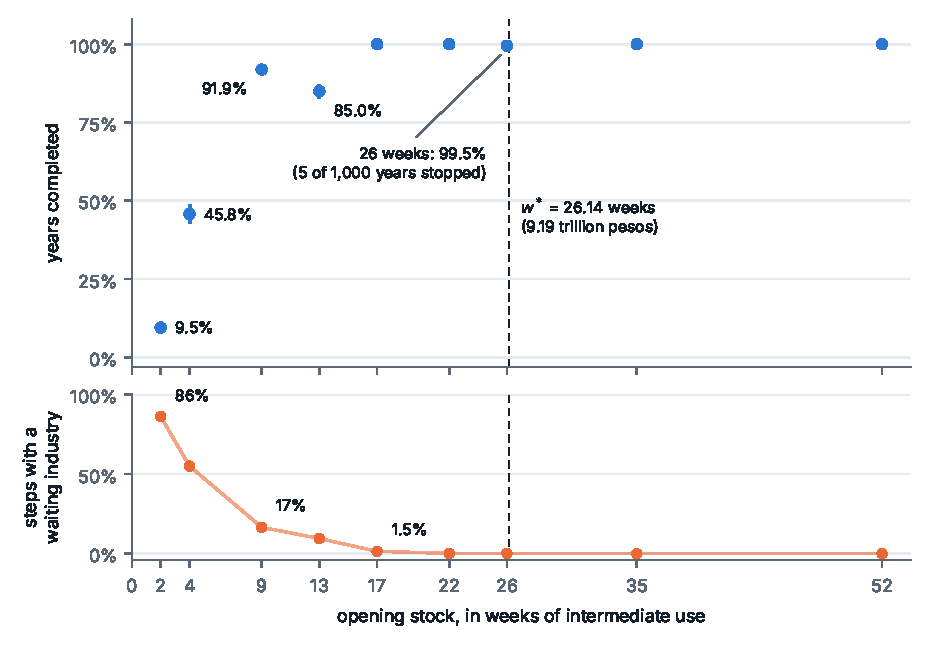
\includegraphics[width=0.92\textwidth]{figures/completion.pdf}
\caption{Top: share of the 1{,}000 simulated years that are completed, by opening stock in weeks of intermediate use, with 95\% Wilson intervals. Bottom: share of steps at which some industry waits. The dashed line is $w^*$ (Table~\ref{tab:minstock}). $N=52$, 80 sectors.}
\label{fig:completion}
\end{figure}

\subsection{The stock that completes every simulated year}

The search started with the interval from 26 weeks, the largest grid stock at which some year stopped, to 35 weeks. None of its six tries had a stopped year (Table~\ref{tab:minstock}), so each try became the new upper end of the interval, and $w^*=26.14$ weeks. This stock is worth 9.19 trillion pesos, about half of a year's intermediate use (18.27 trillion pesos). The 1{,}000 new years at $w^*$ were all completed, so fewer than 3 in 1{,}000 random years stop at $w^*$, with 95\% confidence. This is the preliminary answer to Q1. It does not show that every stock above $w^*$ completes every year: completion is not monotone in the stock, and only the stocks in Tables~\ref{tab:completion} and~\ref{tab:minstock} were tried.

\begin{table}[htbp]
\centering\small
\caption{The answer to Q1 ($N=52$): the search for $w^*$, the smallest stock tried above the largest stock tried at which some year stopped, and its check with 1{,}000 new years.}
\label{tab:minstock}
\begin{tabular}{@{}lcc@{}}
\toprule
& Stock (weeks) & Stopped years (of 1{,}000)\\
\midrule
Search, try 1 & 30.5 & 0\\
Search, try 2 & 28.25 & 0\\
Search, try 3 & 27.125 & 0\\
Search, try 4 & 26.5625 & 0\\
Search, try 5 & 26.28125 & 0\\
Search, try 6 & 26.140625 & 0\\
\midrule
$w^*$ & 26.14 & \\
Value of the stock at $w^*$ & \multicolumn{2}{l}{9.19 trillion pesos}\\
Largest stock tried at which some year stopped & 26 & 5\\
New years at $w^*$ & 26.14 & 0\\
Share of years that stop at $w^*$ & \multicolumn{2}{l}{below 0.3\% (95\% confidence)}\\
\bottomrule
\end{tabular}
\end{table}

\subsection{An order among the completed years}

Table~\ref{tab:order} gives the analysis of the 1{,}000 years at $w^*$, which are the new years of Table~\ref{tab:minstock}; all of them were completed. Waiting is rare at this stock: only 0.6\% of the years had any step at which some industry waited, and on average 0.01\% of the steps of a year had a waiting industry. Without waiting, and with no stopped year left out, there is no reason for an order, and the analysis finds none. No industry fires clearly earlier or later than in the reference years. The ranking from early firings does not agree with the ranking from late firings ($\tau=0.017$, $p=0.82$). None of the 3{,}160 pairs of industries has a significant order, so the timing DAG has no links. The checks on the reference years also find no ordered industry and no link, as they should. At $w^*$, the answer to Q2 is therefore no, as in the small example at $(10,10,13)$.

\begin{table}[htbp]
\centering\small
\caption{Analysis of the firing logs at $w^*$ (1{,}000 years) against the reference years at 52 weeks (1{,}000 years), $N=52$.}
\label{tab:order}
\begin{tabularx}{0.8\textwidth}{@{}Lc@{}}
\toprule
Completed years at $w^*$ & 1{,}000 of 1{,}000\\
Completed years in which some industry waited & 0.6\%\\
Average share of steps with waiting & 0.01\%\\
\addlinespace
Industries clearly earlier / later than the reference & 0 / 0\\
Stability of the sequence, early vs late firings (Kendall's $\tau$) & 0.017 ($p=0.82$)\\
\addlinespace
Links in the timing DAG (of 3{,}160 pairs) & 0\\
Industries on cycles & 0\\
Check: ordered industries and links in the reference years & 0 and 0\\
\bottomrule
\end{tabularx}
\end{table}

\subsection{Single years}

Figure~\ref{fig:years} shows the end of four single simulated years of the 2018 net, from the companion page (Section~\ref{sec:code}). Each row of a grid is one industry, grouped by sector, and each column is one of its 52 batches. A cell is colored when the batch runs, light early in the year and dark late in the year. An orange cell is the next batch of an industry that cannot run when the year stops, and light orange marks the other batches that this industry has left. The line under each grid counts the industries that wait at each step, and the green bar shows the import deliveries that have arrived.

With 52 weeks of stock (panel a), no batch waits, and every row looks the same: the batches of each industry spread evenly over the year. With 9 weeks (b), some industry waits at 39.7\% of the steps, at most 16 industries at the same step, and the year is still completed. With 2 weeks (c), the year stops after 5{,}766 of its 7{,}644 firings: all import deliveries have arrived, 78 industries still have batches left, and 75 of them lack water supply. With 13 weeks (d), the year stops only 30 firings before its end: Electricity and Steam still have batches left, and both lack steam, which only the Steam industry makes, using some steam itself. This is one way in which a larger stock can still stop a year. The analysis of waits and stops (Section~\ref{sec:next}) will show how often it happens.

\begin{figure}[p]
\centering
\begin{subfigure}[t]{0.465\textwidth}\centering
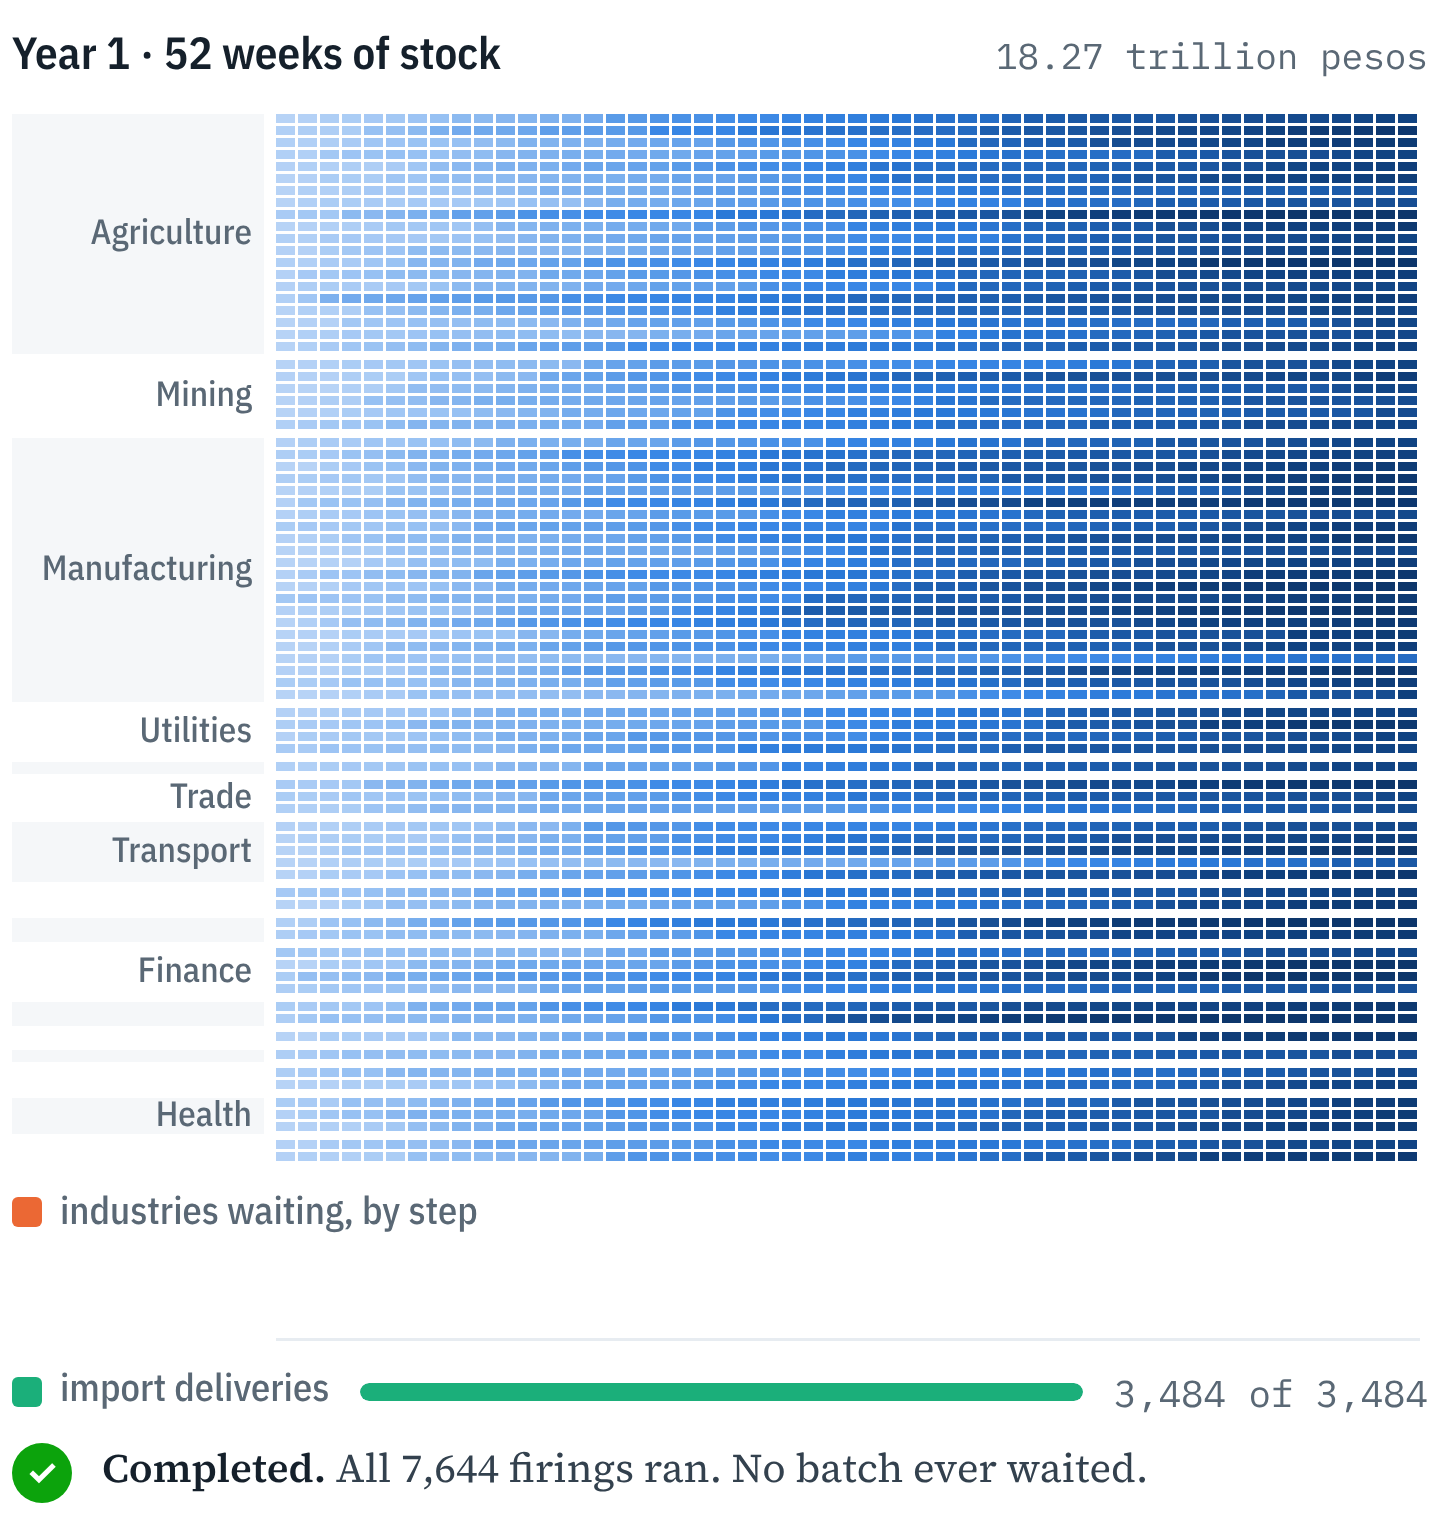
\includegraphics[width=\linewidth]{figures/run_52w.png}
\caption{52 weeks of stock: completed; no batch waited.}
\end{subfigure}\hfill
\begin{subfigure}[t]{0.465\textwidth}\centering
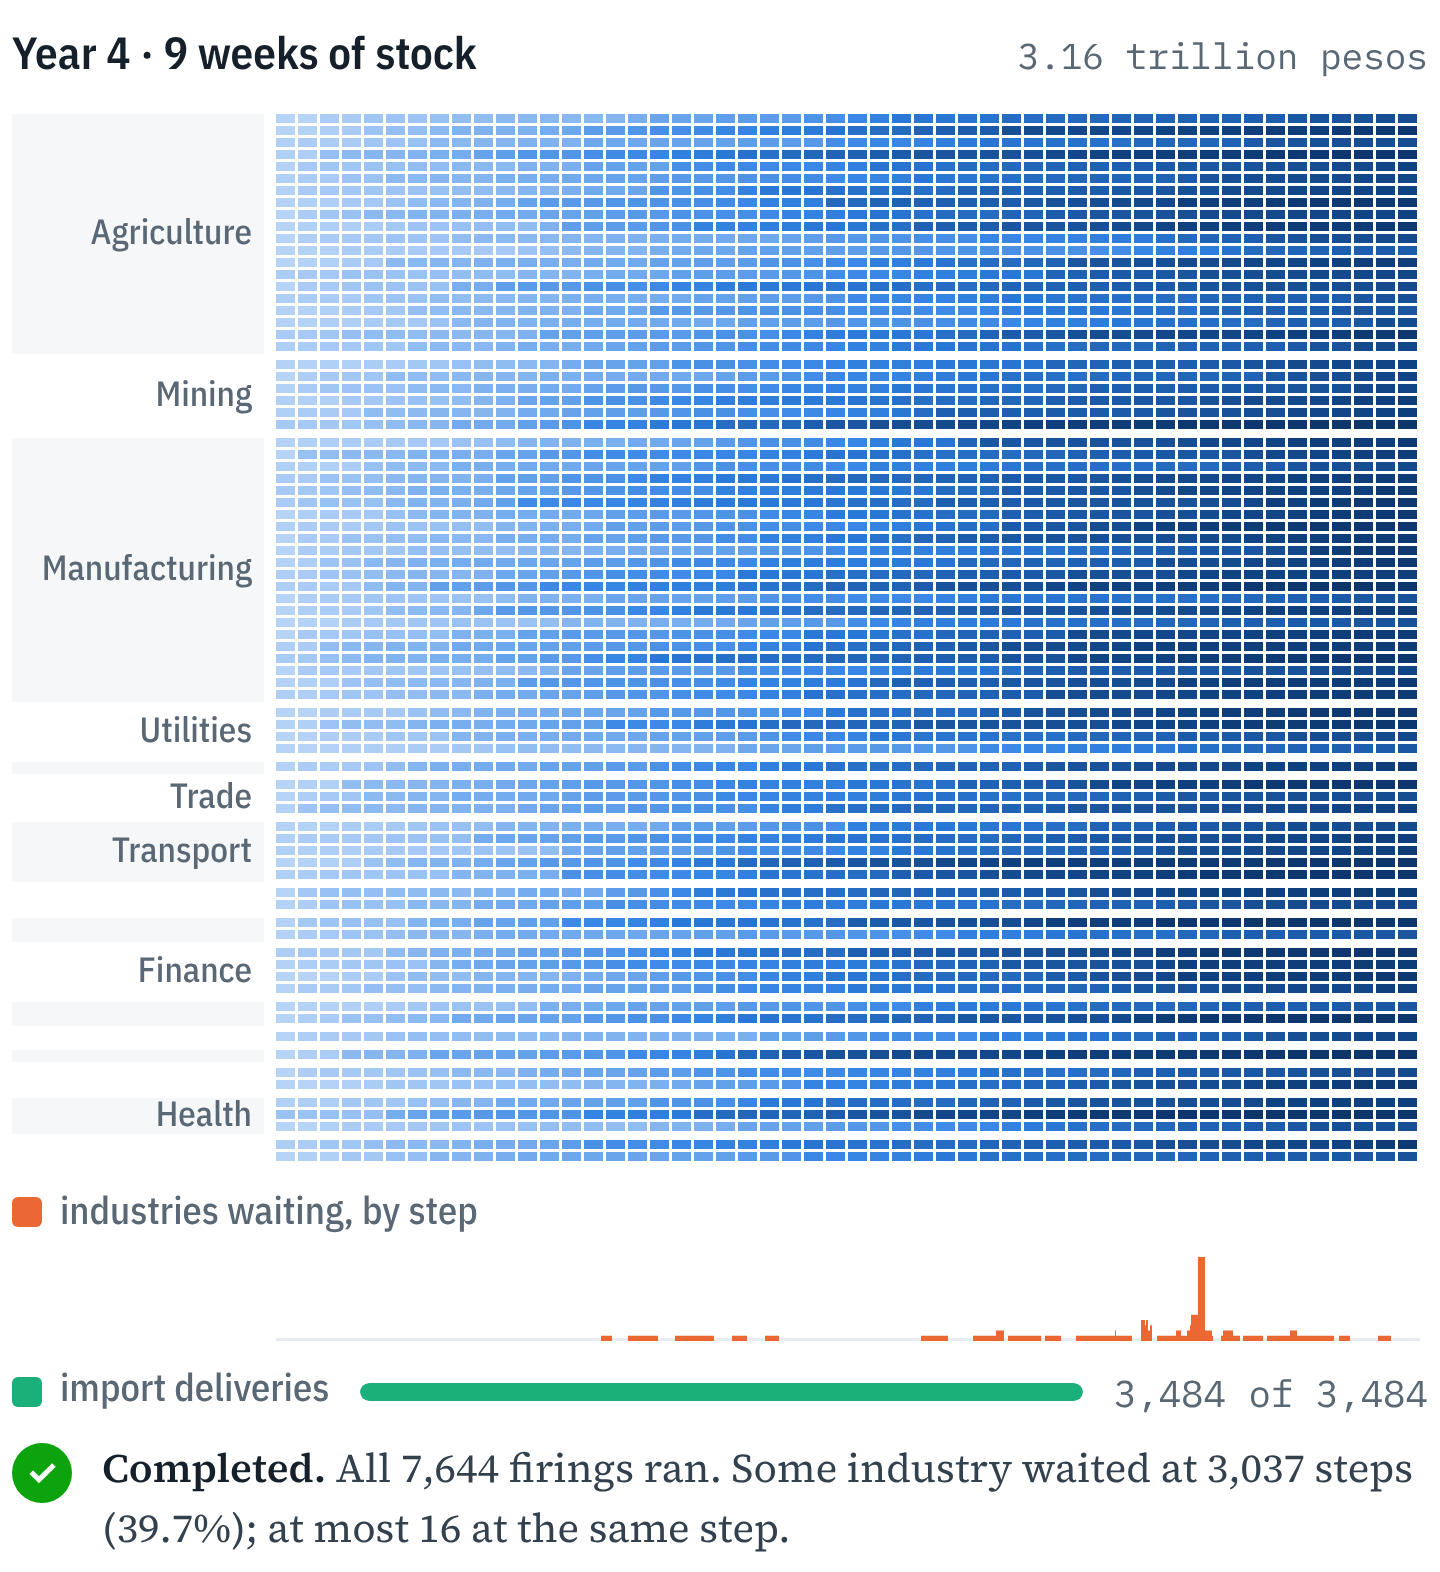
\includegraphics[width=\linewidth]{figures/run_9w.png}
\caption{9 weeks: completed; some industry waited at 39.7\% of the steps.}
\end{subfigure}

\vspace{6pt}
\begin{subfigure}[t]{0.465\textwidth}\centering
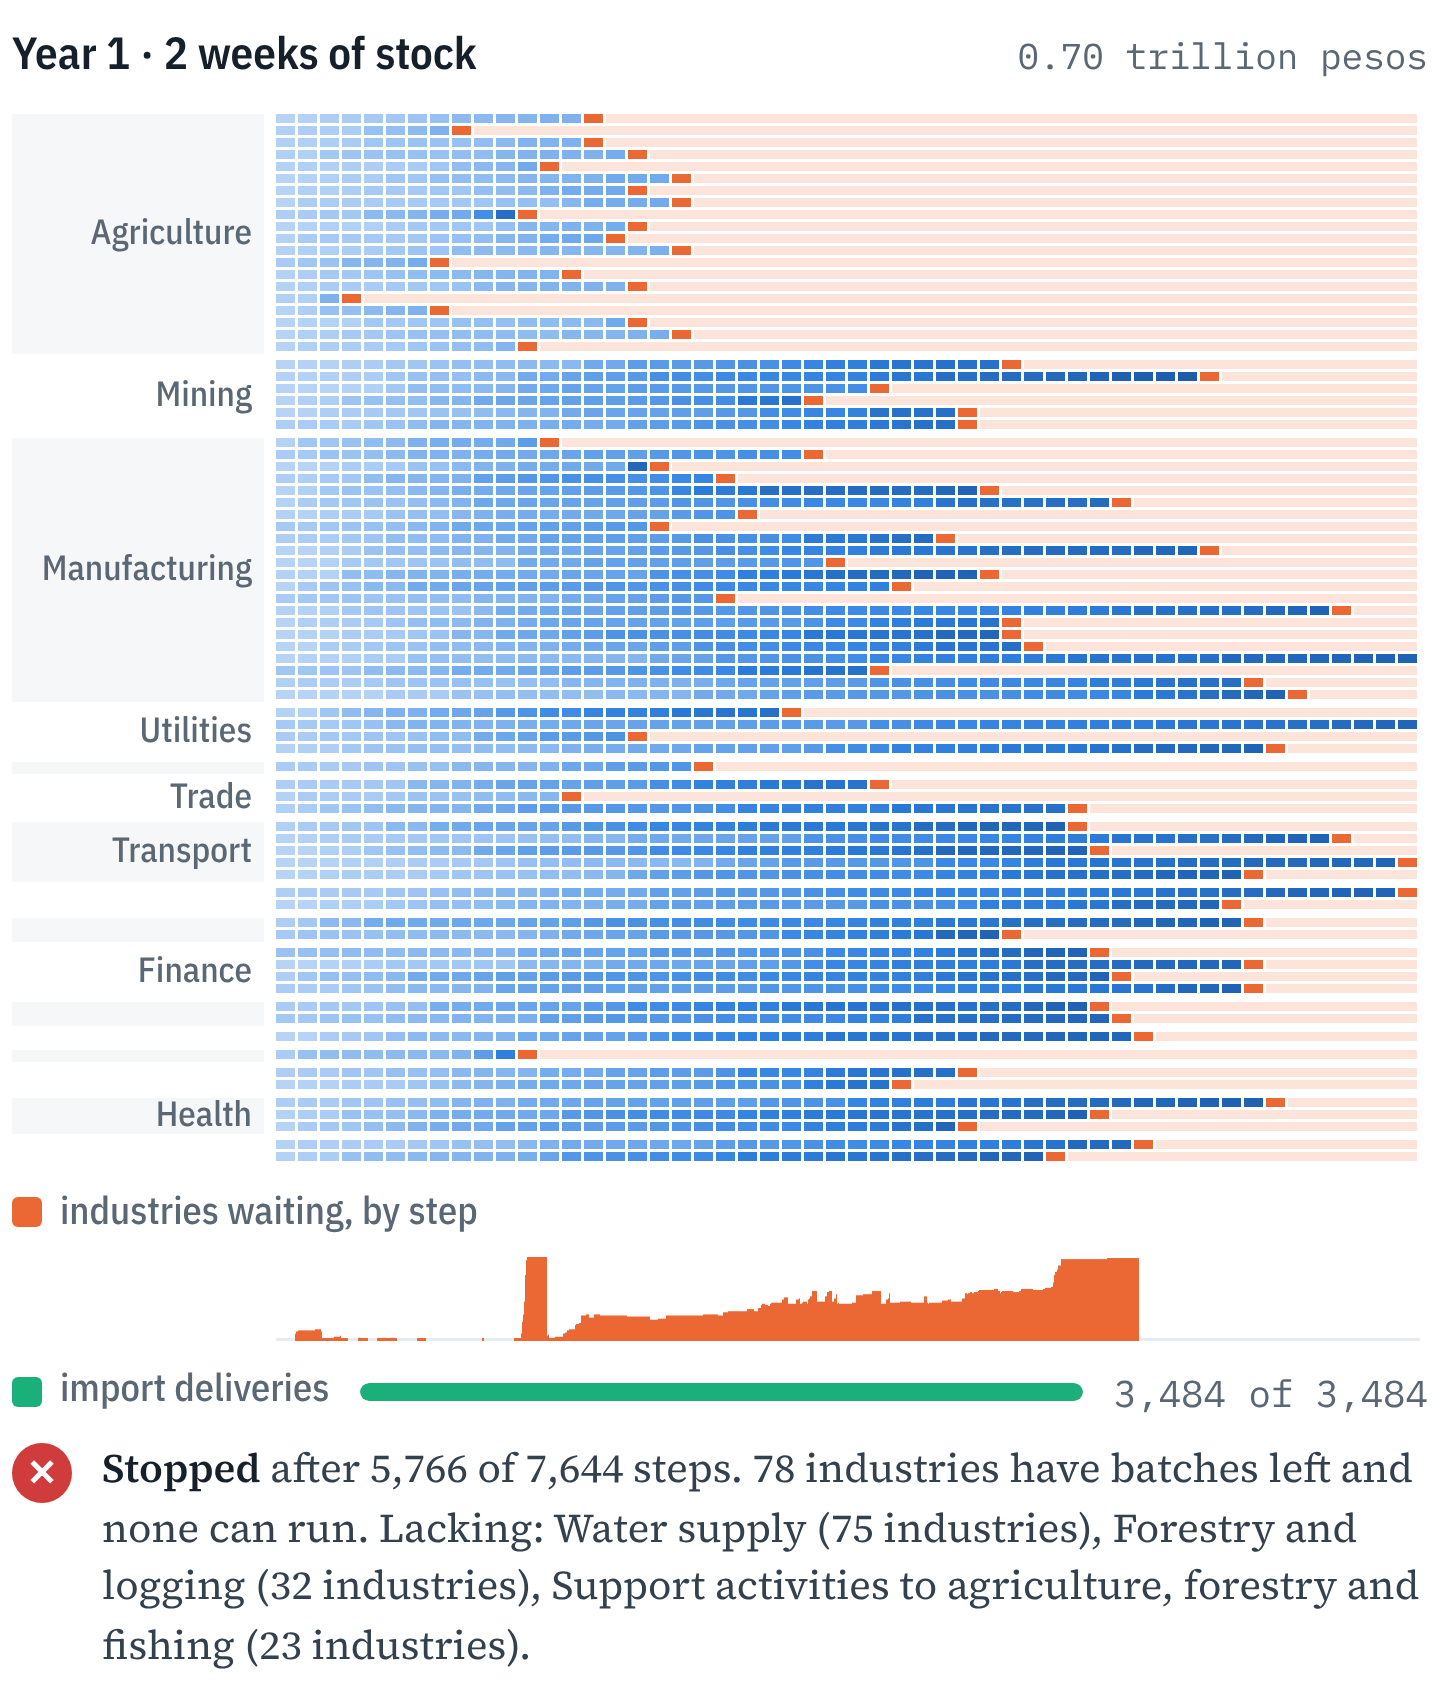
\includegraphics[width=\linewidth]{figures/run_2w.png}
\caption{2 weeks: stopped after 5{,}766 of 7{,}644 firings.}
\end{subfigure}\hfill
\begin{subfigure}[t]{0.465\textwidth}\centering
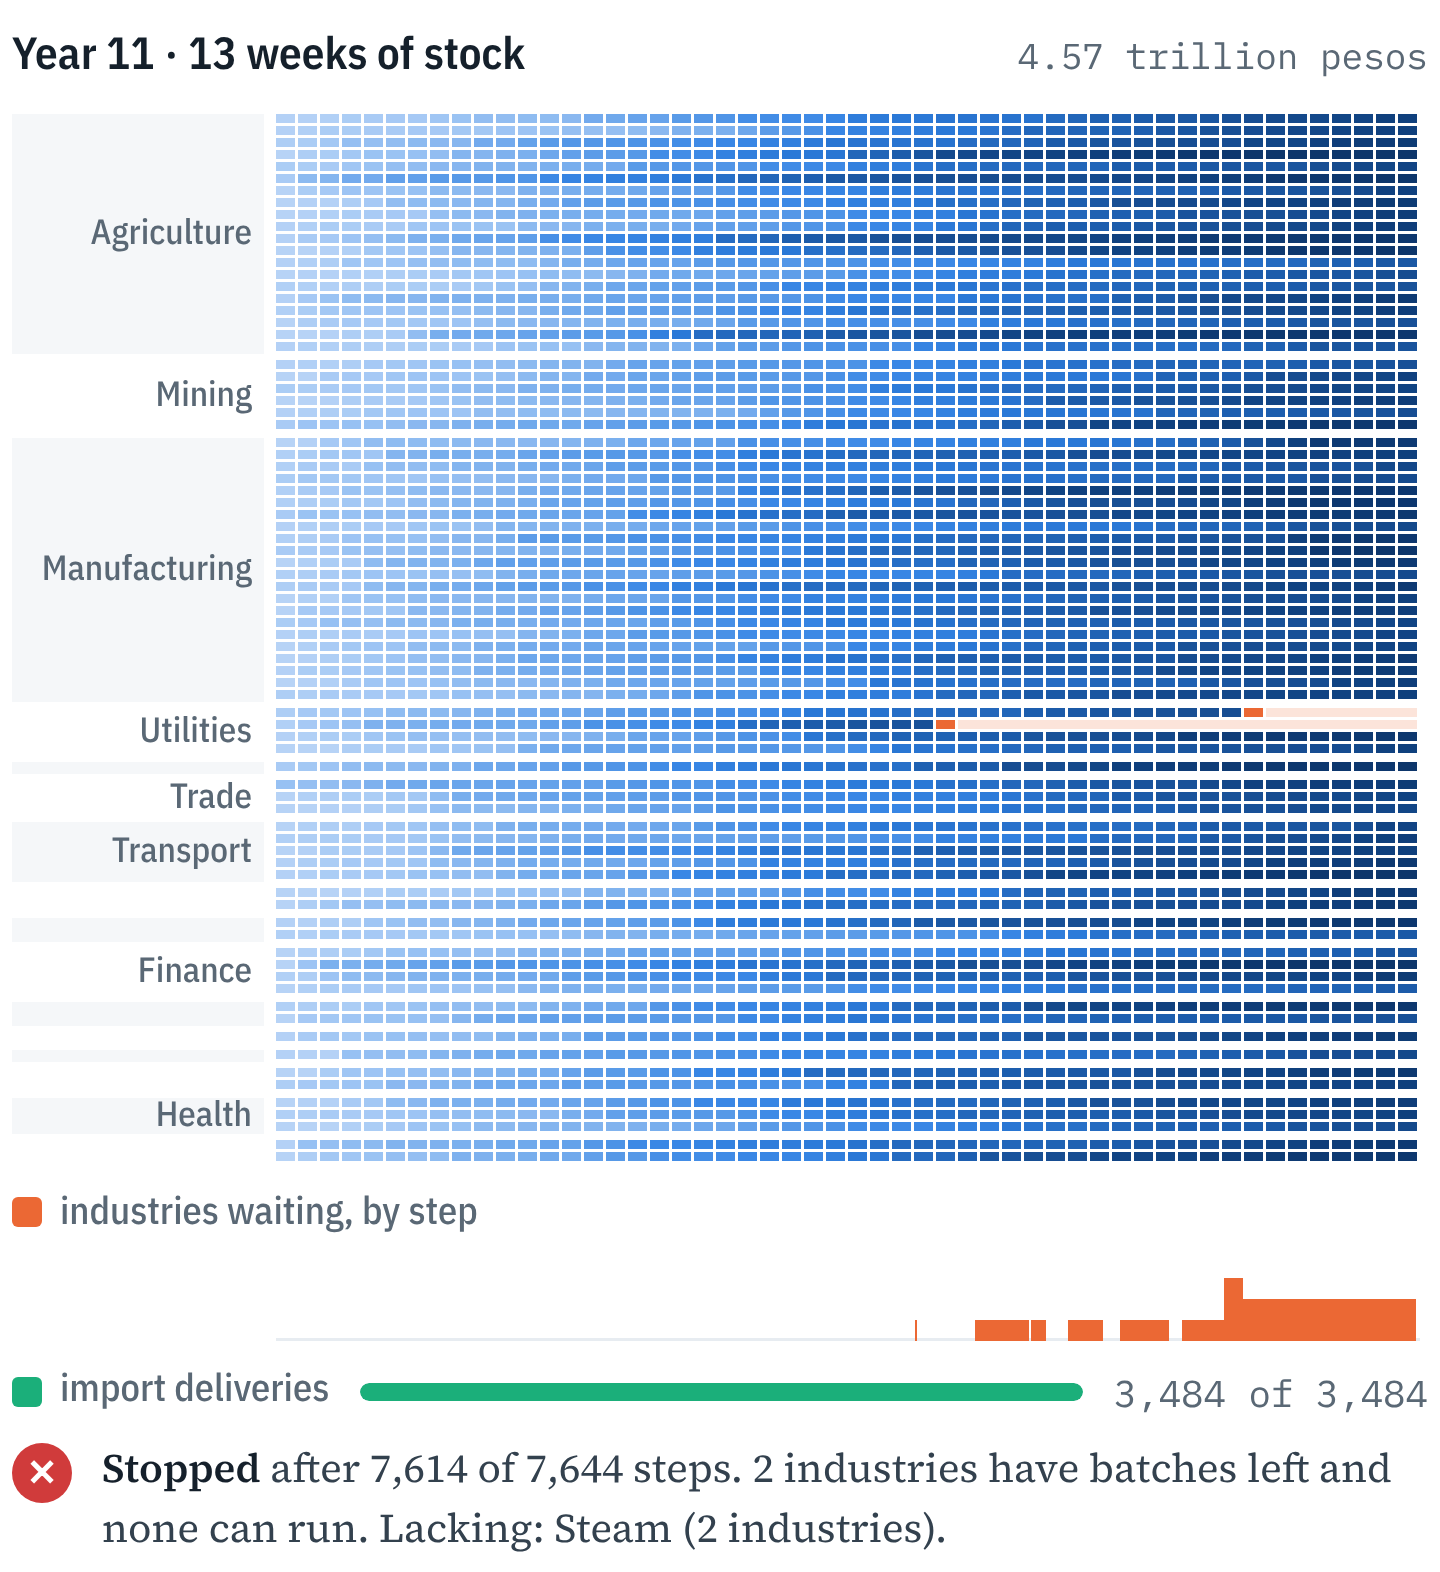
\includegraphics[width=\linewidth]{figures/run_13w.png}
\caption{13 weeks: stopped 30 firings before the end.}
\end{subfigure}
\caption{The end of four simulated years of the 2018 net (80 industries, 52 batches each), from the companion page. Rows are industries, grouped by sector; columns are batches. Blue: batches that ran, from light (early in the year) to dark (late). Orange: the next batch of an industry that cannot run when the year stops; light orange: that industry's other batches left. Under each grid: the number of industries that wait at each step, and the import deliveries. The page uses the year plan and the random rule of the study, with other random numbers.}
\label{fig:years}
\end{figure}

% =====================================================================
\section{Discussion and limitations}\label{sec:discussion}
% =====================================================================

\paragraph{How to read the results.} For Q1, the 80-sector net needs about half a year of intermediate use as opening stock, 26.14 weeks or 9.19 trillion pesos, before every simulated year is completed; with 52 weeks every order completes. Below this, a stopped year proves that the 2018 year could not have been completed in every order that the stock allows: the order of production matters, and the share of completed years says how often a random order still works. Because completion is not monotone in the stock (85.0\% at 13 weeks against 91.9\% at 9 weeks, and rare stops at 26 weeks after none at 17 and 22 weeks), $w^*$ describes the stocks tried; a stock that was not tried, below or above $w^*$, can behave differently. For Q2, the result at $w^*$ is a null result with a clear reason: at this stock industries almost never wait, so the random choice alone sets the order, as in the reference years. An order, if the 2018 table creates one, must be looked for at a stock where industries wait.

\paragraph{Limitations.}
\begin{enumerate}[label=(\roman*),leftmargin=*]
\item \textbf{Values, not physical units.} A token is a unit of product value.
\item \textbf{Fixed recipes and plan.} There is no substitution between inputs, and every industry fires exactly $N$ times in fixed proportions.
\item \textbf{No calendar.} Batches are equal, so there are no seasons; in practice, production in most industries is seasonal \citep{MironZeldes1988}. A batch also uses its inputs and makes its outputs at the same moment.
\item \textbf{Final demand at the end.} Final users take their products only at the closing, so these products stay available to industries during the year, and the stock grows.
\item \textbf{Imports.} Import deliveries need no inputs and can arrive at any time.
\item \textbf{Assumed opening stock.} The table reports changes in inventories but not stock levels. Every product, including services that cannot be stored, gets the same number of weeks.
\item \textbf{Random choice.} The equal chances are a sampling device, so the shares and orders found are properties of the model.
\item \textbf{Statistical answers.} Below 52 weeks, soundness is not proved. $w^*$ depends on the stocks tried, and its 95\% bound comes from the new years at $w^*$, not from the search.
\item \textbf{80 sectors.} Collapsing puts all products of a group into one place, so an industry can use any product of the group, for example any food product. The 80-sector net may therefore need less stock than the 240-sector net; the next draft tests this (Section~\ref{sec:next}).
\item \textbf{One batch size.} Only $N=52$ is used, so the effect of the batch size on the results is not measured.
\item \textbf{One run of the code.} The results come from one run with one seed. The intervals in Table~\ref{tab:completion} show the sampling error of each share.
\end{enumerate}

% =====================================================================
\section{Next steps}\label{sec:next}
% =====================================================================

The next draft extends the study in three ways.

\paragraph{240 sectors.} The code reads PSA's 240-sector tables with one setting (\texttt{SECTORS = 240}). The study will be repeated with 240 products and 240 industries, to see whether the results hold: the shares of completed years by stock, the lower completion at 13 weeks than at 9 weeks, the rare stops near 26 weeks, the value of $w^*$, and the absence of an order at $w^*$. Because collapsing lets an industry use any product of its group, the 240-sector net may need more stock (limitation ix).

\paragraph{An order where industries wait.} The firing logs will be made at a stock where industries wait, such as 9 weeks, where 16.6\% of the steps have a waiting industry and 8.1\% of the years stop. There, an order among the completed years can come from waiting and from the selection of the years that complete (Section~\ref{sec:example}), and the analysis will report both.

\paragraph{Waits and stops.} A new part of the code (\texttt{waits.py} and \texttt{part3\_waits.py}) replays the years of Table~\ref{tab:completion} in their saved order of firings and records every spell of waiting: which industry waited, for which batch, from which step to which step, which firing began the wait (it used an input that was then missing) and which firing ended it (it brought the last missing input). The links ``industry $j$ waited for industry $k$'' form a directed graph. Industries that wait for one another are joined into one group, and the levels of the resulting DAG give an order of dependencies, which can be compared with the timing order of Section~\ref{sec:analysis} and with orders from the structure of the table, such as upstreamness \citep{Antras2012} and triangularization \citep{Fukui1986}. For every stopped year, the replay also shows what holds the year: a group of stuck industries that wait for one another, or an industry that waits for its own product, like Steam in Figure~\ref{fig:years}(d). This part is written and tested, but not yet run.

% =====================================================================
\section{Conclusion}\label{sec:conclusion}
% =====================================================================

The 2018 Philippine SUT records one completed year. Collapsed to 80 sectors, read as a Bonanno production net and closed into a workflow net, it becomes a system in which the order of production matters. Preliminary simulations show that the year can be completed in every simulated order only with a large opening stock: 26.14 weeks of intermediate use, about 9.19 trillion pesos. With less stock, some orders stop, and the share of completed years does not always rise with the stock. At the stock that completes every simulated year, industries almost never wait, and no order of industries appears. The next draft looks for an order where industries wait, records every wait and every stop, and repeats the study with 240 sectors.

% =====================================================================
\section*{Use of AI tools}
% =====================================================================

The literature review, the writing and the coding of this paper were AI-assisted, using Claude Opus 5.5 (Anthropic) and ChatGPT 6 (OpenAI). The conceptualization and the research design are the author's own.

\appendix

% =====================================================================
\section{Reproducing the results}\label{app:reproduce}
% =====================================================================

The code is at \url{https://github.com/miraflor/sut-workflow-study}. It needs Python 3.9 or newer with numpy, scipy, joblib and networkx; matplotlib is optional, and openpyxl is needed only to read the Excel workbooks. The file \texttt{make\_tables.py} saves PSA's 240-sector tables as CSV files. The 80-sector tables come from the workbook \texttt{Philippines\_2018\_80\_Sector\_Observed\_SUT.xlsx}, which adds up PSA's 240-sector tables over PSA's 80 groups; \texttt{make\_tables80.py} saves them as CSV files, and \texttt{aggregate.py} checks them against the 240-sector tables. The file \texttt{settings.py} sets the number of sectors, 52 batches, the stock grid in weeks, the number of runs, the seed and the number of processor cores. Run from a terminal:
\begin{verbatim}
python -m pytest          (the quick checks, less than a minute)
python run.py             (simulations, then analysis)
python run.py runs        (simulations only)
python run.py analysis    (analysis only, from the saved firing logs)
python run.py logs        (firing logs only, at a stock set in LOG_STOCK)
python run.py waits       (waits and stops, at the stocks set in WAIT_STOCKS)
\end{verbatim}
The results are saved in the folder \texttt{results80}:
\begin{itemize}[leftmargin=*]
\item \texttt{table2.csv}, \texttt{search.csv} and \texttt{chosen\_stock.csv}: the results for Q1;
\item \texttt{paths}: the firing logs;
\item \texttt{analysis\_batches52}: \texttt{summary.txt}, the distributions, the sequence and the links of the timing DAG (Q2);
\item \texttt{waits}: one folder per stock, with \texttt{spells.csv}, \texttt{links\_waited\_for.csv}, \texttt{order.csv}, \texttt{stops.csv} and \texttt{summary.txt}.
\end{itemize}
With \texttt{SECTORS = 240} in \texttt{settings.py}, the same commands use PSA's 240-sector tables and save the results in the folder \texttt{results}.

% =====================================================================
\begin{thebibliography}{99}
% =====================================================================

\bibitem[{Antr{\`a}s et~al.}(2012)]{Antras2012}
Antr{\`a}s, P., Chor, D., Fally, T., and Hillberry, R. (2012). Measuring the upstreamness of production and trade flows. \emph{American Economic Review}, 102(3):412--416. \href{https://doi.org/10.1257/aer.102.3.412}{doi:10.1257/aer.102.3.412}.

\bibitem[{Arrow and Debreu}(1954)]{ArrowDebreu1954}
Arrow, K.~J. and Debreu, G. (1954). Existence of an equilibrium for a competitive economy. \emph{Econometrica}, 22(3):265--290.

\bibitem[{Benjamini and Hochberg}(1995)]{BenjaminiHochberg1995}
Benjamini, Y. and Hochberg, Y. (1995). Controlling the false discovery rate: A practical and powerful approach to multiple testing. \emph{Journal of the Royal Statistical Society: Series B}, 57(1):289--300.

\bibitem[{Bonanno}(1993)]{Bonanno1993}
Bonanno, G. (1993). The coverability problem in input--output systems. \emph{Economics Letters}, 43(1):15--21. \href{https://doi.org/10.1016/0165-1765(93)90127-X}{doi:10.1016/0165-1765(93)90127-X}.

\bibitem[{Bonanno}(1995)]{Bonanno1995}
Bonanno, G. (1995). Modeling production with Petri nets. \emph{Economic Notes}, 24(2):263--292.

\bibitem[{Defourny and Thorbecke}(1984)]{DefournyThorbecke1984}
Defourny, J. and Thorbecke, E. (1984). Structural path analysis and multiplier decomposition within a social accounting matrix framework. \emph{Economic Journal}, 94(373):111--136.

\bibitem[{Fukui}(1986)]{Fukui1986}
Fukui, Y. (1986). A more powerful method for triangularizing input-output matrices and the similarity of production structures. \emph{Econometrica}, 54(6):1425--1433.

\bibitem[{Hanley and Lippman-Hand}(1983)]{HanleyLippmanHand1983}
Hanley, J.~A. and Lippman-Hand, A. (1983). If nothing goes wrong, is everything all right? Interpreting zero numerators. \emph{Journal of the American Medical Association}, 249(13):1743--1745.

\bibitem[{Kydland and Prescott}(1982)]{KydlandPrescott1982}
Kydland, F.~E. and Prescott, E.~C. (1982). Time to build and aggregate fluctuations. \emph{Econometrica}, 50(6):1345--1370.

\bibitem[{Leontief}(1936)]{Leontief1936}
Leontief, W.~W. (1936). Quantitative input and output relations in the economic systems of the United States. \emph{Review of Economic Statistics}, 18(3):105--125.

\bibitem[{Miron and Zeldes}(1988)]{MironZeldes1988}
Miron, J.~A. and Zeldes, S.~P. (1988). Seasonality, cost shocks, and the production smoothing models of inventories. \emph{Econometrica}, 56(4):877--908.

\bibitem[{Molina and Guti{\'e}rrez}(2015)]{MolinaGutierrez2015}
Molina, A.~H. and Guti{\'e}rrez, R.~R. (2015). Reformulaci{\'o}n del modelo de Leontief a trav{\'e}s de redes de Petri. \emph{Ciencia y Tecnolog{\'\i}a} (Universidad de Palermo), 15:83--96.

\bibitem[{Murata}(1989)]{Murata1989}
Murata, T. (1989). Petri nets: Properties, analysis and applications. \emph{Proceedings of the IEEE}, 77(4):541--580.

\bibitem[{Philippine Statistics Authority}(2021a)]{PSA2021SUT}
Philippine Statistics Authority (2021a). \emph{2018 Supply and Use Tables} [Excel workbook, as of December 2021]. \url{https://psa.gov.ph/system/files/macroeconomic-accounts/2018\%20Supply\%20and\%20Use\%20Tables.xlsx}.

\bibitem[{Philippine Statistics Authority}(2021b)]{PSA2021Release}
Philippine Statistics Authority (2021b). PSA releases the 2018 Input-Output Tables. 9 December 2021. \url{https://psa.gov.ph/content/psa-releases-2018-input-output-tables}.

\bibitem[{Philippine Statistics Authority}(2021c)]{PSA2021Class}
Philippine Statistics Authority (2021c). \emph{2018 Input-Output Industry Classification} [Excel workbook, as of December 2021]. Released with the 2018 Input-Output Accounts of the Philippines. \url{https://psa.gov.ph/statistics/supply-and-use-input-output/tables}.

\bibitem[{van der Aalst}(1997)]{vanderAalst1997}
van der Aalst, W.~M.~P. (1997). Verification of workflow nets. In \emph{Application and Theory of Petri Nets 1997 (ICATPN 1997)}, Lecture Notes in Computer Science 1248, pages 407--426. Springer.

\bibitem[{van der Aalst}(1998)]{vanderAalst1998}
van der Aalst, W.~M.~P. (1998). The application of Petri nets to workflow management. \emph{Journal of Circuits, Systems and Computers}, 8(1):21--66.

\bibitem[{van der Aalst et~al.}(2011)]{vanderAalst2011}
van der Aalst, W.~M.~P., van Hee, K.~M., ter Hofstede, A.~H.~M., Sidorova, N., Verbeek, H.~M.~W., Voorhoeve, M., and Wynn, M.~T. (2011). Soundness of workflow nets: Classification, decidability, and analysis. \emph{Formal Aspects of Computing}, 23(3):333--363.

\bibitem[{Wilson}(1927)]{Wilson1927}
Wilson, E.~B. (1927). Probable inference, the law of succession, and statistical inference. \emph{Journal of the American Statistical Association}, 22(158):209--212.

\end{thebibliography}

\end{document}
